% !TeX spellcheck = en_US
\addscenariosection{1}{Clash Scenario}{Mines of Moria}{\images/crusader.png}

\begin{multicols*}{2}

\textbf{Author:} LAAMAKALA

\textit{There is no honor — only victory or death. The weak will fall, the strong will fight, and only one will rule.}

\subsection*{\MakeUppercase{Scenario Length}}
This Scenario plays out over 8-12 Rounds.

\subsection*{\MakeUppercase{Player Setup}}
\textbf{Player Count:} 4

\textbf{Starting Resources:} 15 \svg{gold}, 2 \svg{building_materials}, 1 \svg{valuables}

\textbf{Starting Income:} 10 \svg{gold}, 2 \svg{building_materials}, 1 \svg{valuables}

\textbf{Starting Units:}
\begin{itemize}
  \item A Few cheapest \silver\ Units
\end{itemize}

\textbf{Town Buildings:}
\begin{itemize}
  \item \bronze\ Dwelling
  \item City Hall
\end{itemize}

\subsection*{\MakeUppercase{Map Setup}}
Take the following Map Tiles and arrange them as shown in the Scenario map layout ($P$ stands for the number of players):

\begin{itemize}
  \item 4 × Starting (I) Map Tiles
  \item 8 × Far (II-III) Map Tiles
  \item 5 × Near (IV-V) Map Tiles
\end{itemize}

\subsection*{\MakeUppercase{Victory Condition}}
When a player captures their \nth{7} mine all players -- including that player -- take one final turn. After these turns the game ends. The player who controls the most mines is the winner. If there is a tie, the tied player with most \svg{gold} wins.

\subsection*{\MakeUppercase{Timed Events}}
\textbf{\nth{2} Round:}
\begin{itemize}
  \item Players may gain either 10 \svg{gold}, 5 \svg{building_materials} or 2 \svg{valuables}.
\end{itemize}
\textbf{\nth{3} Round:}
\begin{itemize}
  \item Remove all Black Cubes from the Map except Learning Stones.
\end{itemize}
\textbf{\nth{5} Round:}
\begin{itemize}
  \item Repeat the event of Round 3.
\end{itemize}
\textbf{\nth{7} Round:}
\begin{itemize}
  \item Repeat the event of Round 3.
\end{itemize}

\subsection*{\MakeUppercase{Additional Rules}}
\begin{itemize}
  \item Players gain income every Round.
  \item A Secondary Hero starting their turn on I or II-III Map Tile gain +1 \svgeven{movement}.
\end{itemize}

\begin{center}
  \vfill
  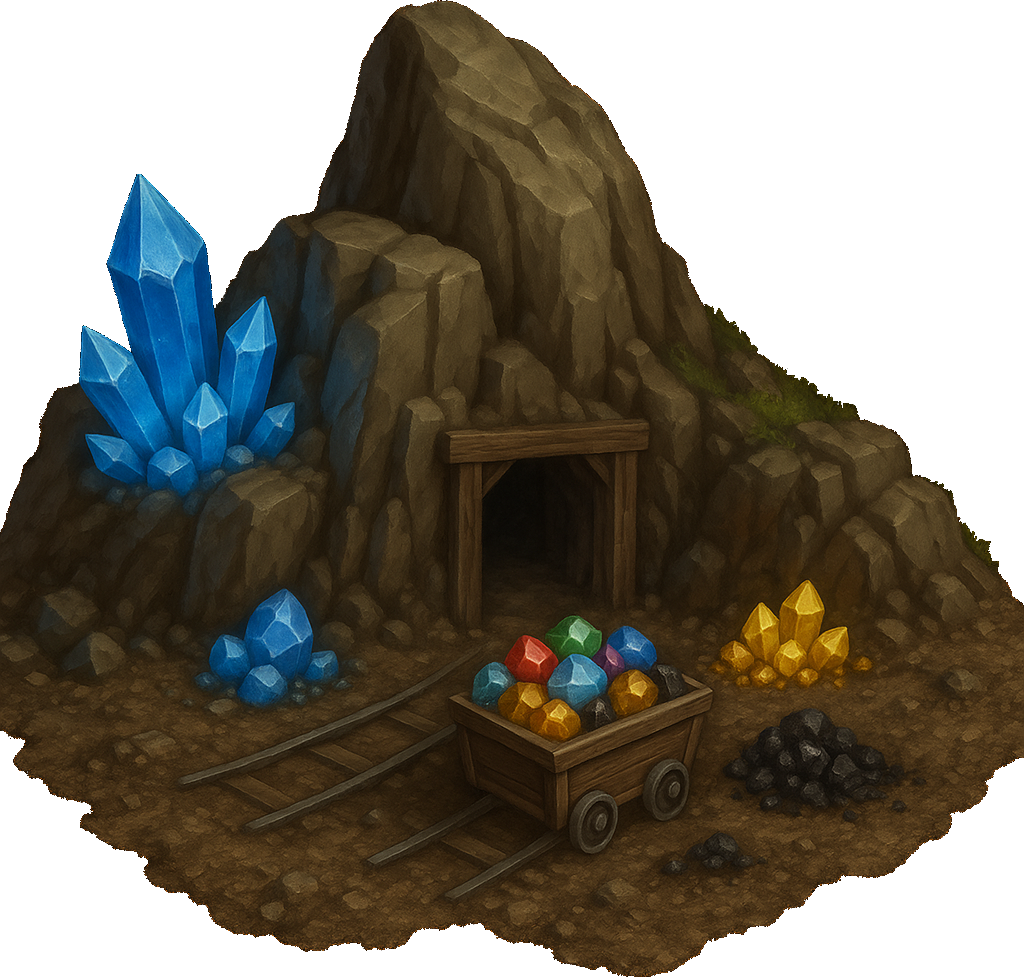
\includegraphics[width=0.95\linewidth]{\maps/mines.png}
  \captionof{figure}{\textbf{SCENARIO MAP LAYOUT}}
  \vfill
\end{center}

\end{multicols*}
